\documentclass{article}
\usepackage{graphicx}
\usepackage[margin=1.5cm]{geometry}
\usepackage{amsmath}

\begin{document}
\twocolumn

\title{Wednesday Warm Up: DC circuits, and Kirchhoff's Rules}
\author{Prof. Jordan C. Hanson}

\maketitle

\section{Memory Bank}

\begin{itemize}
\item $V = I R$ ... Ohm's Law.
\item $P = IV = I^2 R = V^2/R$ ... Power consumption.
\item Kirchhoff's Rule \#1: Total current into a junction equals total current out of a junction.
\item Kirchhoff's Rule \#2: The total change in voltage around a loop is zero.
\end{itemize}

\begin{figure}
\centering
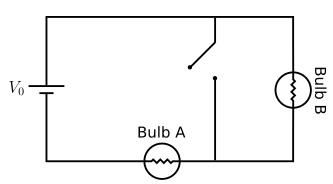
\includegraphics[width=0.4\textwidth]{figures/bulbs.png}
\caption{\label{fig:1} Two light bulbs connected to an EMF $V_0$.}
\end{figure}

\section{Resistors in Series and Parallel, \\ Kirchhoff's Rules}

\begin{enumerate}
\item Consider Fig. \ref{fig:1}.  (a) If $V_0 = 12$ V, and the resistances of bulbs A and B are $5$ $\Omega$, what current flows if the switch in the middle is open? (b) What current flows if the switch is closed, and through which bulb? \textit{Hint: be careful, because the the total current into a junction equals the total output current.} \\ \vspace{5cm}
\item For the system in Fig. \ref{fig:1}, what is the power consumption if the switch is (a) open, (b) closed? \\ \vspace{3cm}
\item Consider Fig. \ref{fig:2}.  Let $V_1 = 12$ V, $V_2 = 1.2$ V, and all resistors have a value of $2$ $\Omega$.  Solve for the currents through all resistors.
\end{enumerate}

\begin{figure}
\centering
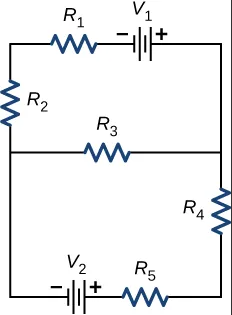
\includegraphics[width=0.225\textwidth,trim=0cm 0cm 0.1cm 0.0cm,clip=true]{figures/kirchhoff_3.png}\caption{\label{fig:2} A circuit with two batteries and five resistors.}
\end{figure}

\end{document}
